\chapter{Evaluation}\label{chap:evaluation}

This section reflects the results of all the testing performed with the different programming languages and architectures / types of computer.

\begin{table}[ht]
  \centering
  \begin{tabular}{lcccc}
    \toprule
                            & C\++                  & Go        & Python        & PyPy \\
    \midrule
    Intel Xeon Gold 6326 x2 &  GCC 14.2.0           & go1.24.2  & Python 3.12.3 & PyPy 7.3.19 \\
    MacbookPro M4 Pro       &  Apple Clang 17.0.0   & go1.24.2  & Python 3.13.3 & PyPy 7.3.19 \\
    Raspberry Pi 5          &                       &           &               &             \\
    Ryzen 3800x Desktop     &                       &           &               &             \\
    \bottomrule
  \end{tabular}
  \caption{Comparison of language performance on different platforms}
  \label{tab:lang-platforms}
\end{table}

It should be noted that Python should not be used for performance-critical applications, as it is an interpreted language and is not designed for high-performance computing. However, it is an excellent language for rapid prototyping and development, and it is widely used in the industry.

Go's intent is to be a fast, efficient, and easy-to-use language. It is designed for multithreading and concurrency, which makes it a great choice for high-performance computing. Go was specifically designed for backend development for web applications and is widely used in the industry.

\section{Measurement Platforms}

\subsection{Many-Core Platform}

This platform represents the most powerful as well as power-hungry combination of all devices in my test suite. This is a rack server with two Intel Xeon Gold 6326 processors, each having 16 cores and 32 threads, contributing to a total of 32 cores and 64 threads. It also has the largest amount of \gls{ram} from this testing, with 256GB of \gls{DDR4} memory.

As it has two sockets (one per CPU chip), there must be intercommunication between these processors if a process spreads out to more than 32 threads, or is set by the user using the command \texttt{taskset}, which fixes the cores the process can run on.



%% Comments on the platform, ie two xeon 16 cores processors with hyperthreading, x86
\subsubsection{Evaluated Parameters}

This system was the most versatile in terms of the number of tests that could be performed, as it has many processors and uses Linux on x86, providing a great advantage for forcing processes to run on specific cores.

The tests were conducted on a variety of core configurations, always setting cores in the same processor for core numbers less than 16.

\begin{itemize}
    \item \textbf{1 Core}: Testing with one core, producing the baseline for the program's energy consumption and execution time.
    \item \textbf{2 Cores}: Testing with 2 cores provides the first glimpse of parallelization benefits.
    \item \textbf{4 Cores}: Testing with 4 cores because many computers from some time ago had four cores.
    \item \textbf{8 Cores}: Testing with 8 cores gives us great insight into how many processors in the market work, and it is half the amount of cores inside one chip.
    \item \textbf{14 Cores}: Testing with 14 cores, because it is the number of cores available on the laptop and we wanted to have an execution time comparison.
    \item \textbf{16 Cores}: Testing with 16 cores as it is the amount of real cores on a single chip. This should be one of the most energy-efficient and fastest tests, if there were only one \gls{cpu}.
    \item \textbf{28 Cores (different \glspl{cpu}, all real cores, no logical cores)}: Testing with 28 cores distributed across two sockets is interesting because there has to be information sharing over the bus inside the motherboard to synchronize both \glspl{cpu}. This won't be as energy efficient, but may be faster.
    \item \textbf{28 Cores (same CPU, 16 cores, 32 virtual cores)}: Testing with 28 cores inside the same CPU; the performance should be slower as there are fewer real cores to tackle the work, but it has the advantage of not needing to share data with another socket.
    \item \textbf{32 Cores (same socket)}: Testing with 32 cores in the same socket uses all available logical threads of a system: the 16 real cores and the other 16 threads the \gls{cpu} has thanks to Hyper-Threading.
    \item \textbf{32 Cores (only real cores)}: Testing with 32 real cores across two sockets should be the most powerful combination for CPU-intensive tasks, as all operations should be able to be carried out without many interruptions.
    \item \textbf{48 Cores}: Testing with 48 cores forces us to use all real cores and some logical cores.
    \item \textbf{60 Cores}: Testing with 60 cores is also interesting (not 64), as this would force the machine to interrupt the program we are benchmarking to perform routine operations, such as checking for incoming connections or logging.
\end{itemize}

\subsubsection{Results}

The results for the server are shown in the following figures and tables. The energy consumption is measured in joules, and the execution time is measured in seconds. 

\begin{figure}[H]
  \centering
  \begin{tikzpicture}
  \begin{semilogyaxis}[
      title={Logarithmic energy (pkg) consumption - Server},
      width=\plotwidthgraph,
      height=\plotheightgraph,
      xlabel={Number of Cores},
      ylabel={Energy (J)},
      ymode=log,
      xmode=linear,
      grid=both,
      minor tick num=1,
      grid style={gray!30,dashed},
      xtick={1,2,4,8,14,16,28,32,48,60},
      x tick label style={
        font=\footnotesize,
        rotate=45,
        anchor=north east
      },
      legend style={
        at={(0.98,0.98)},
        anchor=north east,
        font=\scriptsize,
        nodes={scale=0.8,transform shape},
        draw=none
      },
      legend columns=2,
      transpose legend,
      legend cell align=left,
    ]

    %% C++ %%
    % open circles
    \addplot[
      blue,
      only marks,
      mark=o,
      mark options={draw=blue,fill=white}
    ] table[row sep=\\] {
      x    y \\
      1    3756.26  \\
      2    2591.91  \\
      4    1362.61  \\
      8    799.23   \\
      14   603.37   \\
      16   627.16   \\
      28   541.37   \\  
      32   529.61   \\  
      48   740.57   \\
      60   666.04   \\
    };
    \addlegendentry{C++}
    % filled circles at 28 & 32
    \addplot[
      blue,
      only marks,
      mark=*,
      mark options={draw=blue,fill=blue}
    ] table[row sep=\\] {
      x    y \\
      28   766.51   \\  
      32   757.79   \\  
    };
    \addlegendentry{C++ same CPU}
    % trendline, but do NOT add to legend:
    \addplot[
      blue,
      dashed,
      forget plot,
      domain=1:60,
      samples=200
    ] {3000 * x^(-0.4513)};

    %% Go %%
    \addplot[
      violet,
      only marks,
      mark=o,
      mark options={draw=violet,fill=white}
    ] table[row sep=\\] {
      x    y \\
      1    28522.69 \\
      2    18231.97 \\
      4    10304.27	\\
      8    5617.27  \\
      14   3155.30  \\
      16   2904.52  \\
      28   2306.35  \\
      32   2151.74  \\
      48   1856.93  \\
      60   1744.76  \\
    };
    \addlegendentry{Go}
    \addplot[
      violet,
      only marks,
      mark=*,
      mark options={draw=violet,fill=violet}
    ] table[row sep=\\] {
      x    y \\
      28   2271.71  \\
      32   2109.37  \\
    };
    \addlegendentry{Go same CPU}
    \addplot[
      violet,
      dashed,
      forget plot,
      domain=1:60,
      samples=200
    ] {23600 * x^(-0.6783)};

    %% PyPy %%
    \addplot[
      orange,
      only marks,
      mark=o,
      mark options={draw=orange,fill=white}
    ] table[row sep=\\] {
      x    y \\
      1    7972.65  \\
      2    5147.60  \\
      4    2828.21  \\
      8    1747.96  \\
      14   1232.03  \\
      16   1140.80  \\
      28   1252.93  \\
      32   1257.81  \\
      48   1354.03  \\
      60   1354.03  \\
    };
    \addlegendentry{PyPy}
    \addplot[
      orange,
      only marks,
      mark=*,
      mark options={draw=orange,fill=orange}
    ] table[row sep=\\] {
      x    y \\
      28   1175.52  \\
      32   1155.74  \\
    };
    \addlegendentry{PyPy same CPU}
    \addplot[
      orange,
      dashed,
      forget plot,
      domain=1:60,
      samples=200
    ] {6250 * x^(-0.4633)};

    %% Python %%
    \addplot[
      green!60!black,
      only marks,
      mark=o,
      mark options={draw=green!60!black,fill=white}
    ] table[row sep=\\] {
      x    y \\
      1    1510534.76 \\
      2    1141490.15 \\
      4    313537.85  \\
      8    194458.98  \\
      14   130506.94  \\
      16   111438.01  \\
      28   122384.40  \\
      32   120259.78  \\
      48   97331.00   \\
      60   93718.97   \\
    };
    \addlegendentry{Python}
    \addplot[
      green!60!black,
      only marks,
      mark=*,
      mark options={draw=green!60!black,fill=green!60!black}
    ] table[row sep=\\] {
      x    y \\
      28   96049.86 \\  
      32   87343.61 \\
    };
    \addlegendentry{Python same CPU}
    \addplot[
      green!60!black,
      dashed,
      forget plot,
      domain=1:60,
      samples=200
    ] {1.27e6 * x^(-0.7046)};

  \end{semilogyaxis}
\end{tikzpicture}
\caption{Server - Logarithmic energy (pkg) consumption}{Logarithm energy (pkg) consumption of the Server benchmark across different programming languages.}
\label{fig:log-server-energy-pkg}
\end{figure}


\begin{figure}[h]
  \centering
  \begin{tikzpicture}
  \begin{axis}[
      title={Energy efficiency speedup},
      width=\plotwidthgraph,
      height=\plotheightgraph,
      xlabel={Number of Cores},
      ylabel={Speedup (relative to 1 core)},
      xmode=linear,
      grid=both,
      minor tick num=1,
      grid style={gray!30,dashed},
      xtick={1,2,4,8,14,16,28,32,48,60},
      x tick label style={
        font=\footnotesize,
        rotate=45,
        anchor=north east
      },
      legend style={
        at={(0.02,0.98)},
        anchor=north west,
        font=\scriptsize,
        nodes={scale=0.8,transform shape},
        draw=none
      },
      legend columns=1,
      legend cell align=left,
      ymin=0,
      ymax=18,
    ]

    %% C++ Speedup (Energy efficiency improvement) %%
    \addplot[
      blue,
      mark=o,
      mark options={draw=blue,fill=white},
      line width=1.5pt
    ] table[row sep=\\] {
      x    y \\
      1    1.00  \\
      2    1.45  \\
      4    2.76  \\
      8    4.70  \\
      14   6.22  \\
      16   5.99  \\
      28   6.94  \\  
      32   7.09  \\  
      48   5.07  \\
      60   5.64  \\
    };
    \addlegendentry{C++}
    
    \addplot[
      blue,
      only marks,
      mark=*,
      mark options={draw=blue,fill=blue}
    ] table[row sep=\\] {
      x    y \\
      28   4.90  \\  
      32   4.95  \\  
    };
    \addlegendentry{C++ same CPU}

    %% Go Speedup %%
    \addplot[
      violet,
      mark=o,
      mark options={draw=violet,fill=white},
      line width=1.5pt
    ] table[row sep=\\] {
      x    y \\
      1    1.00  \\
      2    1.56  \\
      4    2.77  \\
      8    5.08  \\
      14   9.04  \\
      16   9.82  \\
      28   12.37 \\
      32   13.26 \\
      48   15.36 \\
      60   16.35 \\
    };
    \addlegendentry{Go}
    
    \addplot[
      violet,
      only marks,
      mark=*,
      mark options={draw=violet,fill=violet}
    ] table[row sep=\\] {
      x    y \\
      28   12.56 \\
      32   13.52 \\
    };
    \addlegendentry{Go same CPU}

    %% PyPy Speedup %%
    \addplot[
      orange,
      mark=o,
      mark options={draw=orange,fill=white},
      line width=1.5pt
    ] table[row sep=\\] {
      x    y \\
      1    1.00  \\
      2    1.55  \\
      4    2.82  \\
      8    4.56  \\
      14   6.47  \\
      16   6.99  \\
      28   6.36  \\
      32   6.34  \\
      48   5.89  \\
      60   5.89  \\
    };
    \addlegendentry{PyPy}
    
    \addplot[
      orange,
      only marks,
      mark=*,
      mark options={draw=orange,fill=orange}
    ] table[row sep=\\] {
      x    y \\
      28   6.78  \\
      32   6.90  \\
    };
    \addlegendentry{PyPy same CPU}

    %% Python Speedup %%
    \addplot[
      green!60!black,
      mark=o,
      mark options={draw=green!60!black,fill=white},
      line width=1.5pt
    ] table[row sep=\\] {
      x    y \\
      1    1.00  \\
      2    1.32  \\
      4    4.82  \\
      8    7.77  \\
      14   11.57 \\
      16   13.55 \\
      28   12.34 \\
      32   12.56 \\
      48   15.52 \\
      60   16.11 \\
    };
    \addlegendentry{Python}
    
    \addplot[
      green!60!black,
      only marks,
      mark=*,
      mark options={draw=green!60!black,fill=green!60!black}
    ] table[row sep=\\] {
      x    y \\
      28   15.73 \\  
      32   17.29 \\
    };
    \addlegendentry{Python same CPU}

  \end{axis}
  \end{tikzpicture}
\caption{Server - Speedup Energy Efficiency}{Server benchmark energy performance comparison across programming languages: Energy efficiency speedup relative to single-core performance (higher is better).}
\label{fig:energy-comparison}
\end{figure}


\begin{figure}
  \centering
  \begin{tikzpicture}
  \begin{semilogyaxis}[
      title={Logarithmic energy (ram) consumption - Server},
      width=\plotwidthgraph,
      height=\plotheightgraph,
      xlabel={Number of Cores},
      ylabel={Energy (J)},
      ymode=log,
      xmode=linear,
      grid=both,
      minor tick num=1,
      grid style={gray!30,dashed},
      xtick={1,2,4,8,14,16,28,32,48,60},
      x tick label style={
        font=\footnotesize,
        rotate=45,
        anchor=north east
      },
      legend style={
        at={(0.98,0.98)},
        anchor=north east,
        font=\scriptsize,
        nodes={scale=0.8,transform shape},
        draw=none
      },
      legend columns=2,
      transpose legend,
      legend cell align=left,
    ]

    %% C++ %%
    \addplot[
      blue,
      only marks,
      mark=o,
      mark options={draw=blue,fill=white}
    ] table[row sep=\\] {
      x    y \\
      1    176.83  \\
      2    111.08  \\
      4    67.60   \\
      8    26.28   \\
      14   18.28   \\
      16   19.29   \\
      28   16.91   \\
      32   17.80   \\
      48   27.02   \\
      60   24.40   \\
    };
    \addlegendentry{C++}
    \addplot[
      blue,
      only marks,
      mark=*,
      mark options={draw=blue,fill=blue}
    ] table[row sep=\\] {
      x    y \\
      28   29.01   \\
      32   28.15   \\
    };
    \addlegendentry{C++ same CPU}
    % power‐law fit: y = 138.9 * x^(–0.5506)
    \addplot[
      blue,
      forget plot,
      domain=1:60,
      samples=200
    ] {128.71 * x^(-0.540)};

    %% Go %%
    \addplot[
      violet,
      only marks,
      mark=o,
      mark options={draw=violet,fill=white}
    ] table[row sep=\\] {
      x    y \\
      1    1049.92 \\
      2    755.43  \\
      4    426.69  \\
      8    175.15  \\
      14   107.26  \\
      16   95.60   \\
      28   55.09   \\
      32   61.70   \\
      48   85.73   \\
      60   90.01   \\
    };
    \addlegendentry{Go}
    \addplot[
      violet,
      only marks,
      mark=*,
      mark options={draw=violet,fill=violet}
    ] table[row sep=\\] {
      x    y \\
      28   78.01   \\
      32   65.66   \\
    };
    \addlegendentry{Go same CPU}
    % power‐law fit: y = 1024.9 * x^(–0.7437)
    \addplot[
      violet,
      forget plot,
      domain=1:60,
      samples=200
    ] {975.38 * x^(-0.728)};

    %% PyPy %%
    \addplot[
      orange,
      only marks,
      mark=o,
      mark options={draw=orange,fill=white}
    ] table[row sep=\\] {
      x    y \\
      1    355.42  \\
      2    253.06  \\
      4    170.08  \\
      8    88.94   \\
      14   72.28   \\
      16   71.84   \\
      28   81.44   \\
      32   83.50   \\
      48   89.06   \\
      60   91.31   \\
    };
    \addlegendentry{PyPy}
    \addplot[
      orange,
      only marks,
      mark=*,
      mark options={draw=orange,fill=orange}
    ] table[row sep=\\] {
      x    y \\
      28   78.81   \\
      32   77.79   \\
    };
    \addlegendentry{PyPy same CPU}
    % power‐law fit: y = 292.4 * x^(–0.3661)
    \addplot[
      orange,
      forget plot,
      domain=1:60,
      samples=200
    ] {273.36 * x^(-0.357)};

    %% Python %%
    \addplot[
      green!60!black,
      only marks,
      mark=o,
      mark options={draw=green!60!black,fill=white}
    ] table[row sep=\\] {
      x    y \\
      1    59269.48 \\
      2    36442.43 \\
      4    12799.44 \\
      8    6683.08  \\
      14   4031.07  \\
      16   3705.32  \\
      28   4057.46  \\
      32   4037.98  \\
      48   2850.62  \\
      60   2703.02  \\
    };
    \addlegendentry{Python}
    \addplot[
      green!60!black,
      only marks,
      mark=*,
      mark options={draw=green!60!black,fill=green!60!black}
    ] table[row sep=\\] {
      x    y \\
      28   2831.52 \\
      32   2576.33 \\
    };
    \addlegendentry{Python same CPU}
    % power‐law fit: y = 4.79e4 * x^(–0.7649)
    \addplot[
      green!60!black,
      forget plot,
      domain=1:60,
      samples=200
    ] {45451.50 * x^(-0.760)};

  \end{semilogyaxis}
\end{tikzpicture}
\caption{Server - Logarithmic energy (ram) consumption}{Logarithm energy (ram) consumption of the Server benchmark across different programming languages.}
\label{fig:log-server-energy-ram}
\end{figure}




\begin{figure}
  \centering

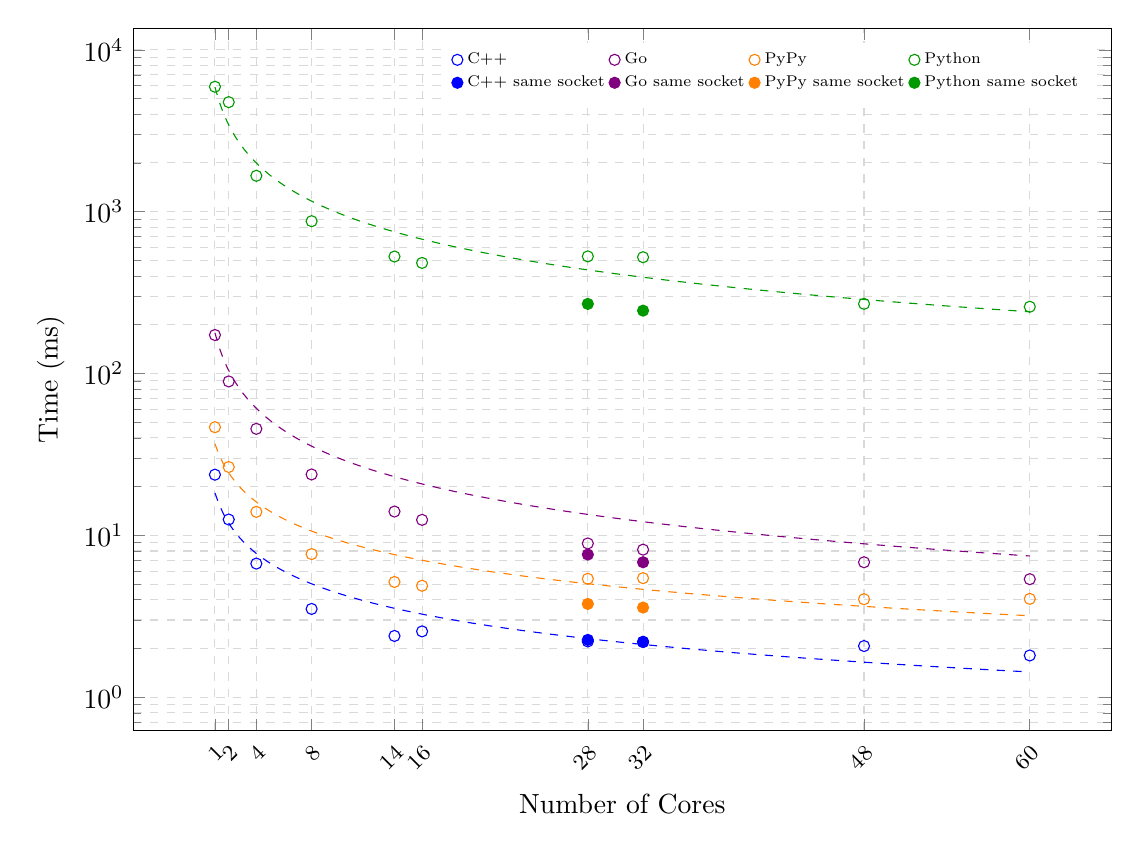
\begin{tikzpicture}
  \begin{semilogyaxis}[
      width=14cm,
      height=10.5cm,
      xlabel={Number of Cores},
      ylabel={Time (ms)},
      ymode=log,
      xmode=linear,
      grid=both,
      minor tick num=1,
      grid style={gray!30,dashed},
      xtick={1,2,4,8,14,16,28,32,48,60},
      x tick label style={
        font=\footnotesize,
        rotate=45,
        anchor=north east
      },
      legend style={
        at={(0.98,0.98)},
        anchor=north east,
        font=\scriptsize,
        nodes={scale=0.8,transform shape},
        draw=none
      },
      legend columns=2,
      transpose legend,
      legend cell align=left,
    ]

    %% C++ %%
    \addplot[
      blue,
      only marks,
      mark=o,
      mark options={draw=blue,fill=white}
    ]
    table[row sep=\\] {
      x    y \\
      1    23.70  \\
      2    12.52  \\
      4    6.69   \\
      8    3.51   \\
      14   2.39   \\
      16   2.55   \\
      28   2.21   \\
      32   2.20   \\
      48   2.07   \\
      60   1.81   \\
    };
    \addlegendentry{C++}

    \addplot[
      blue,
      only marks,
      mark=*,
      mark options={draw=blue,fill=blue}
    ]
    table[row sep=\\] {
      x    y \\
      28   2.26   \\
      32   2.19   \\
    };
    \addlegendentry{C++ same socket}

    % power‐law fit: y = 18.3 * x^(-0.6223)
    \addplot[
      blue,
      dashed,
      forget plot,
      domain=1:60,
      samples=200
    ] {18.3 * x^(-0.6223)};

    %% Go %%
    \addplot[
      violet,
      only marks,
      mark=o,
      mark options={draw=violet,fill=white}
    ]
    table[row sep=\\] {
      x    y \\
      1    172.952 \\
      2    89.32  \\
      4    45.51  \\
      8    23.78  \\
      14   14.03  \\
      16   12.46  \\
      28   8.91   \\
      32   8.16   \\
      48   6.82   \\
      60   5.36   \\
    };
    \addlegendentry{Go}

    \addplot[
      violet,
      only marks,
      mark=*,
      mark options={draw=violet,fill=violet}
    ]
    table[row sep=\\] {
      x    y \\
      28   7.61  \\
      32   6.82  \\
    };
    \addlegendentry{Go same socket}

    % power‐law fit: y = 178.3 * x^(-0.7753)
    \addplot[
      violet,
      dashed,
      forget plot,
      domain=1:60,
      samples=200
    ] {178.3 * x^(-0.7753)};

    %% PyPy %%
    \addplot[
      orange,
      only marks,
      mark=o,
      mark options={draw=orange,fill=white}
    ]
    table[row sep=\\] {
      x    y \\
      1    46.58  \\
      2    26.43  \\
      4    13.97  \\
      8    7.66   \\
      14   5.15   \\
      16   4.88   \\
      28   5.39   \\
      32   5.44   \\
      48   4.03   \\
      60   4.05   \\
    };
    \addlegendentry{PyPy}

    \addplot[
      orange,
      only marks,
      mark=*,
      mark options={draw=orange,fill=orange}
    ]
    table[row sep=\\] {
      x    y \\
      28   3.77   \\
      32   3.58   \\
    };
    \addlegendentry{PyPy same socket}

    % power‐law fit: y = 36.8 * x^(-0.5976)
    \addplot[
      orange,
      dashed,
      forget plot,
      domain=1:60,
      samples=200
    ] {36.8 * x^(-0.5976)};

    %% Python %%
    \addplot[
      green!60!black,
      only marks,
      mark=o,
      mark options={draw=green!60!black,fill=white}
    ]
    table[row sep=\\] {
      x    y \\
      1    5913.41  \\
      2    4749.55  \\
      4    1665.41  \\
      8    872.89   \\
      14   528.12   \\
      16   482.30   \\
      28   529.22   \\
      32   523.04   \\
      48   269.41   \\
      60   258.44   \\
    };
    \addlegendentry{Python}

    \addplot[
      green!60!black,
      only marks,
      mark=*,
      mark options={draw=green!60!black,fill=green!60!black}
    ]
    table[row sep=\\] {
      x    y \\
      28   269.13  \\
      32   244.57  \\
    };
    \addlegendentry{Python same socket}

    % power‐law fit: y = 5894 * x^(-0.7811)
    \addplot[
      green!60!black,
      dashed,
      forget plot,
      domain=1:60,
      samples=200
    ] {5894 * x^(-0.7811)};

  \end{semilogyaxis}
\end{tikzpicture}

\caption{Execution time of the server in Joules for different core configurations}
  \label{fig:server-execution-time}
\end{figure}

\begin{table}[ht]
    \centering
    \begin{tabular}{lrrrr}
        \hline
        time         & C++             & Go            & PyPy          & Python     \\
        \hline
        1            & 23.70           & 172.952       & 46.58         & 5,913.41        \\
        2            & 12.52           & 89.32         & 26.43         & 4,749.55        \\
        4            & 6.69            & 45.51         & 13.97         & 1,665.41        \\
        8	           & 3.51  	         & 23.78 	       & 7.66          & 872.89          \\
        14           & 2.39            & 14.03         & 5.15          & 528.12          \\
        16           & 2.55            & 12.46         & 4.88          & 482.30          \\
        28           & 2.21            & 8.91          & 5.39          & 529.22          \\
        28 same CPU  & 2.26            & 7.61          & 3.77          & 269.13          \\
        32           & 2.20            & 8.16          & 5.44          & 523.04          \\
        32 same CPU  & 2.19            & 6.82          & 3.58          & \textbf{244.57} \\
        48           & 2.07            & 6.82          & 4.03          & 269.41          \\
        60           & \textbf{1.81}   & \textbf{5.36} & \textbf{4.05} & 258.44          \\
        \hline
    \end{tabular}
    \caption{Execution time by implementation and core count}
    \label{tab:server-execution-time}
\end{table}



From \autoref{fig:server-energy-pkg}, we can see that the energy consumption of the server is not linear with the number of cores. It can be observed that the energy consumption decreases as the number of cores increases, but there is a point in the graph and \autoref{tab:server-energy-pkg} where the energy consumption starts to increase slightly again, as well as the execution times in \autoref{fig:server-execution-time}, but not as much as the energy consumption.

This is due to hyperthreading\footnote{Hyperthreading is enabled in this system as it is not mine and I cannot disable it to perform testing. To set the process to a fixed \gls{cpu}, I used \texttt{taskset -c [cores]}, i.e., \texttt{taskset -c 0-15,32-47} for running across multiple \glspl{cpu} and \texttt{taskset -c 0-31} to force the program to only run in a single \gls{cpu}.} in the \glspl{cpu}, which allows the \glspl{cpu} to run two threads per core, but this is not as efficient as running a single thread per core, as the \glspl{cpu} have to share resources between the two threads.

It is obvious from the multiple graphs and tables that the C\++ implementation is the most energy-efficient and fastest by a significant margin, followed surprisingly by the PyPy execution of the Python code, which is faster than the Go implementation, and the Python implementation is the slowest and most energy-consuming by an extremely large amount.

However, when looking closely at the 28-core and 32-core tests, focusing on C\++, we can see the energy consumption is lower when using cores from different CPUs rather than consuming more, as there is some energy efficiency loss when synchronizing the data between the two CPUs. What happens in this case is that the C\++ parallelization algorithm makes each of the cores have a very hard \gls{cpu} workload, resulting in a more efficient result. This aligns with \autoref{sec:hyperthreading}, where it is explained that hyperthreading is not as efficient for specific tasks.

I want to specifically discuss the 60-core test, as it is the most interesting one. In this test, the energy consumption is lower than in the 48-core test, as well as the execution time on the C\++ implementation, but on the Go implementation, both energy consumption and execution time are higher than in the 48-core test. This is because the Go implementation is not as efficient as the C\++ implementation, and the Go runtime has to manage more goroutines, which adds overhead.

Considering the 32-core and 48-core tests with the Python program, the energy consumption reduces significantly when the program starts using virtual cores, as the program is able to run on more cores, and the Python runtime is not very demanding, being able to use these cores efficiently. As shown in \autoref{fig:server-energy-pkg} and \autoref{fig:server-execution-time}, this is an advantage to Python with respect to itself.





\begin{figure}
    \centering
    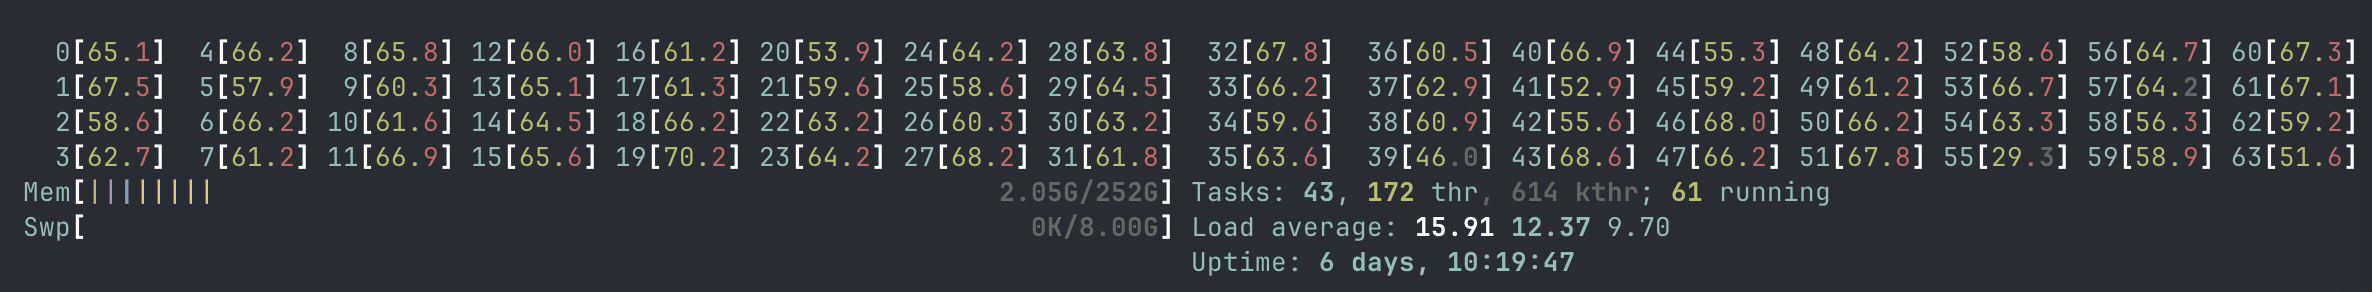
\includegraphics[width=1\linewidth]{img/htop_not_running_100_60_cores.png}
    \caption{\gls{htop} showing the cores not being used at 100\% when using many cores for processing in a per-pixel multi threading renderer }
    \label{fig:htop_60_not_100}
\end{figure}

It also must be noted that the cores during the 48 core benchmark were being used at 100\% of their capacity, while in the 60 cores test, the cores were mostly being usead at a lower percentage, as shown in \autoref{fig:htop_60_not_100}. This is because the Go runtime is not able to efficiently use all the cores when there are more than 48 cores available, and it is not able to schedule the goroutines efficiently as these routines finish so fast that the Go runtime is not able to keep all the cores busy.

If we changed the implementation to a per-row renderer, on the go-side, the Go runtime would be able to use all the cores more efficiently, as it would be able to schedule the goroutines more efficiently, and the execution time would be lower, but the energy consumption would be higher, as the cores would be used at 100\% of their capacity. Thus, in this case, as we will see in other sections, having a faster execution time is not always the best option in terms of energy consumption.


% When changin to a per-pixel rendered, lower cores energy efficiency increased, but the many cores, from 48 oward would not get used as much, thus reducing the energy efficiency and increating the execution time. 



\subsection{Personal Desktop}
%% Comments on the platform x86, 8 cores, 16 threads, AMR ZEN 2 (https://www.amd.com/en/support/downloads/drivers.html/processors/ryzen/ryzen-3000-series/amd-ryzen-7-3800x.html#amd_support_product_spec)
%% Test with and without hyerthreading as math intensive calculations
\subsubsection{Evaluated parameters}
\subsubsection{Results}

\subsection{Personal SOTA Laptop}
This lapot is said to have one of the fastest single-core performance in the market. It has a 14 core ARM processor, using the big.LITTLE architecture, with 10 high performance cores and 4 high efficiency cores. It has 48GB of RAM, which is enough to run any of the tests.


\subsubsection{Evaluated parameters}

This platform is a personal laptop, with a 14 core processor, the Apple M4 Pro, which has 10 high performance cores and 4 high efficiency cores, which is a big.LITTLE architecture. This means that the high performance cores are used for CPU intensive tasks, while the high efficiency cores are used for less demanding tasks, such as web browsing or watching videos. But as Apple does not allow the user seting the cores to be used by a specific process, like it happens in Linux, we can not test the high efficiency cores isolated from the high performance cores, as the operating system will decide for us which cores to use for each process. 



\subsubsection{Results}

\begin{figure}
    \centering
    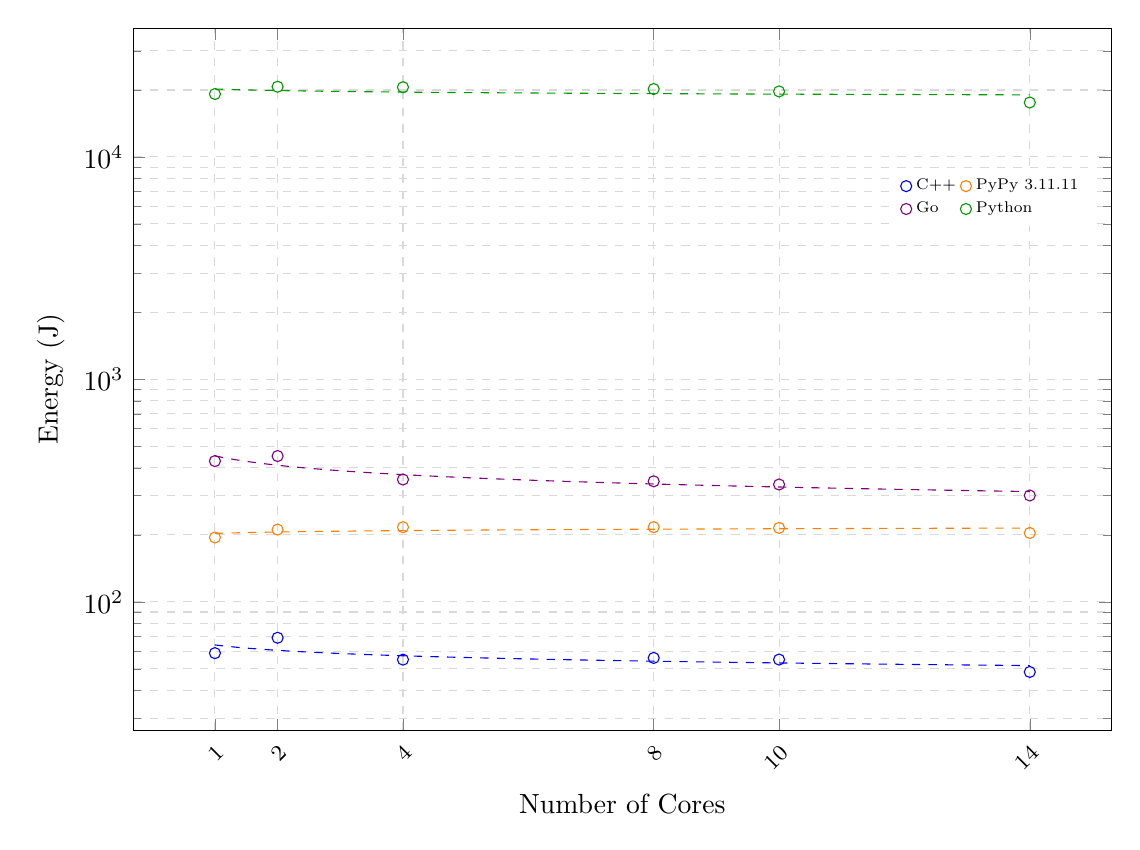
\begin{tikzpicture}
    %% Add a title for the figure
  \begin{semilogyaxis}[
      width=14cm,
      height=10.5cm,
      xlabel={Number of Cores},
      ylabel={Energy (J)},
      ymode=log,
      xmode=linear,
      grid=both,
      minor tick num=1,
      grid style={gray!30,dashed},
      xtick={1,2,4,8,10,14},
      x tick label style={
        font=\footnotesize,
        rotate=45,
        anchor=north east
      },
      legend style={
        at={(0.98,0.8)},
        anchor=north east,
        font=\scriptsize,
        nodes={scale=0.8,transform shape},
        draw=none
      },
      legend columns=2,
      transpose legend,
      legend cell align=left,
    ]
    %% C++ %%
    \addplot[
      blue,
      only marks,
      mark=o,
      mark options={draw=blue,fill=white}
    ]
    table[row sep=\\] {
      x    y      \\
      1    58.79  \\
      2    68.93  \\
      4    54.97  \\
      8    55.94  \\
      10   55.00  \\
      14   48.39  \\
    };
    \addlegendentry{C++}
    % power‐law fit: y = 64.0 * x^(–0.081)
    \addplot[
      blue,
      dashed,
      forget plot,
      domain=1:14,
      samples=200
    ] {64.0 * x^(-0.081)};

    %% Go %%
    \addplot[
      violet,
      only marks,
      mark=o,
      mark options={draw=violet,fill=white}
    ]
    table[row sep=\\] {
      x     y       \\
      1     429.23  \\
      2     452.12  \\
      4     354.64  \\
      8     348.14  \\
      10    336.88  \\
      14    300.66  \\
    };
    \addlegendentry{Go}
    % power‐law fit: y = 453 * x^(–0.140)
    \addplot[
      violet,
      dashed,
      forget plot,
      domain=1:14,
      samples=200
    ] {453 * x^(-0.140)};

    %% PyPy 3.11.11 %%
    \addplot[
      orange,
      only marks,
      mark=o,
      mark options={draw=orange,fill=white}
    ]
    table[row sep=\\] {
      x    y      \\
      1    194.69 \\
      2    211.21 \\
      4    216.53 \\
      8    216.60 \\
      10   214.96 \\
      14   203.92 \\
    };
    \addlegendentry{PyPy 3.11.11}
    % power‐law fit: y = 203 * x^(0.021)
    \addplot[
      orange,
      dashed,
      forget plot,
      domain=1:14,
      samples=200
    ] {203 * x^(0.021)};

    %% Python %%
    \addplot[
      green!60!black,
      only marks,
      mark=o,
      mark options={draw=green!60!black,fill=white}
    ]
    table[row sep=\\] {
      x      y        \\
      1      19183.95 \\
      2      20680.94 \\
      4      20580.73 \\
      8      20198.35 \\
      10     19701.50 \\
      14     17567.03 \\
    };
    \addlegendentry{Python}
    % power‐law fit: y = 20200 * x^(–0.023)
    \addplot[
      green!60!black,
      dashed,
      forget plot,
      domain=1:14,
      samples=200
    ] {20200 * x^(-0.023)};

  \end{semilogyaxis}
\end{tikzpicture}
    \caption{Logarithm Energy consumption of the MBP algorithm in different programming languages.}
    \label{fig:log-mbp-energy}
\end{figure}

\begin{figure}
    \centering
    
    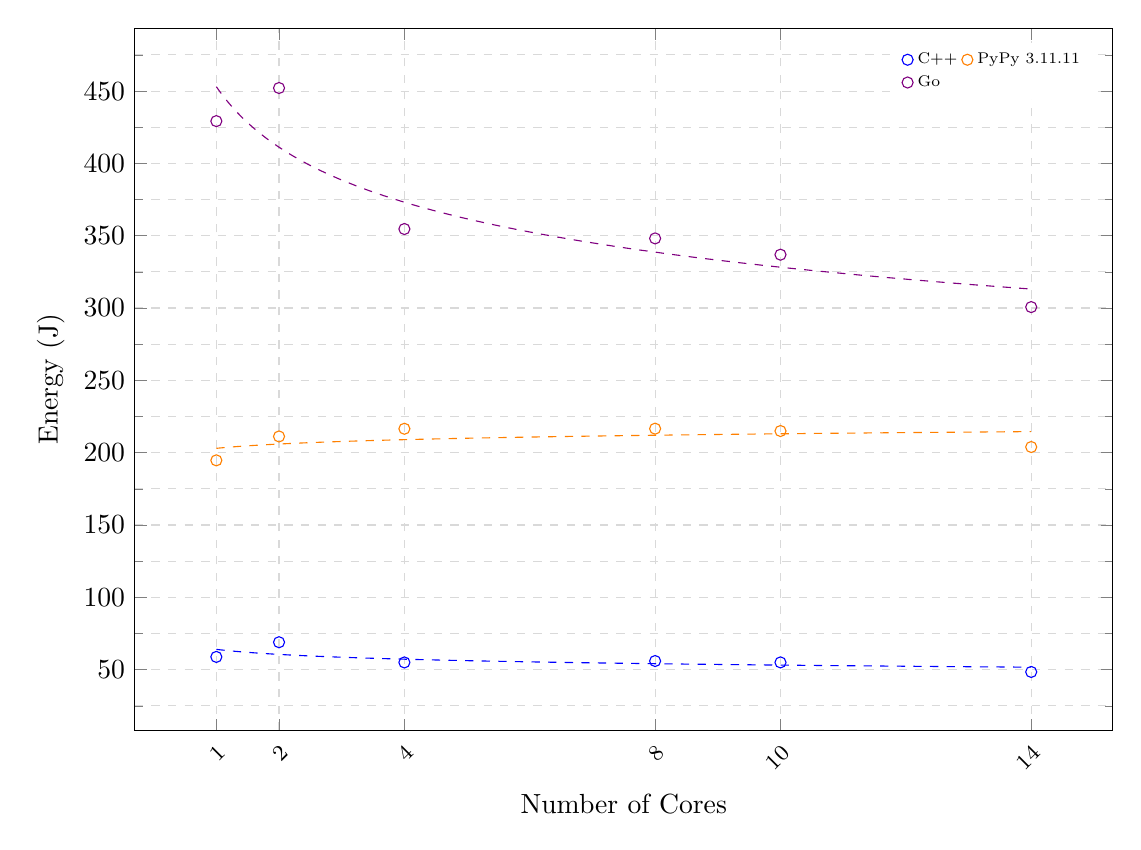
\begin{tikzpicture}
  \begin{axis}[
      width=14cm,
      height=10.5cm,
      xlabel={Number of Cores},
      ylabel={Energy (J)},
      ymode=linear,
      xmode=linear,
      grid=both,
      minor tick num=1,
      grid style={gray!30,dashed},
      xtick={1,2,4,8,10,14},
      x tick label style={
        font=\footnotesize,
        rotate=45,
        anchor=north east
      },
      legend style={
        at={(0.98,0.98)},
        anchor=north east,
        font=\scriptsize,
        nodes={scale=0.8,transform shape},
        draw=none
      },
      legend columns=2,
      transpose legend,
      legend cell align=left,
    ]
    %% C++ %%
    \addplot[
      blue,
      only marks,
      mark=o,
      mark options={draw=blue,fill=white}
    ]
    table[row sep=\\] {
      x    y      \\
      1    58.79  \\
      2    68.93  \\
      4    54.97  \\
      8    55.94  \\
      10   55.00  \\
      14   48.39  \\
    };
    \addlegendentry{C++}
    % power‐law fit: y = 64.0 * x^(–0.081)
    \addplot[
      blue,
      dashed,
      forget plot,
      domain=1:14,
      samples=200
    ] {64.0 * x^(-0.081)};

    %% Go %%
    \addplot[
      violet,
      only marks,
      mark=o,
      mark options={draw=violet,fill=white}
    ]
    table[row sep=\\] {
      x     y       \\
      1     429.23  \\
      2     452.12  \\
      4     354.64  \\
      8     348.14  \\
      10    336.88  \\
      14    300.66  \\
    };
    \addlegendentry{Go}
    % power‐law fit: y = 453 * x^(–0.140)
    \addplot[
      violet,
      dashed,
      forget plot,
      domain=1:14,
      samples=200
    ] {453 * x^(-0.140)};

    %% PyPy 3.11.11 %%
    \addplot[
      orange,
      only marks,
      mark=o,
      mark options={draw=orange,fill=white}
    ]
    table[row sep=\\] {
      x    y      \\
      1    194.69 \\
      2    211.21 \\
      4    216.53 \\
      8    216.60 \\
      10   214.96 \\
      14   203.92 \\
    };
    \addlegendentry{PyPy 3.11.11}
    % power‐law fit: y = 203 * x^(0.021)
    \addplot[
      orange,
      dashed,
      forget plot,
      domain=1:14,
      samples=200
    ] {203 * x^(0.021)};

  \end{axis}
\end{tikzpicture}

    \caption{Linear Energy consumption of the MBP algorithm in different programming languages.}
    \label{fig:linear-mbp-energy}
\end{figure}

\begin{table}
    \centering
    \begin{tabular}{lrrrr}
        \hline
        Cores & C++   & Go     & PyPy 3.11.11 & Python      \\
        \hline
        1     & 58.79  & 429.23  & 194.69       & 19,183.95   \\
        2     & 68.93  & 452.12  & 211.21       & 20,680.94   \\
        4     & 54.97  & 354.64  & 216.53       & 20,580.73   \\
        8     & 55.94  & 348.14  & 216.60       & 20,198.35   \\
        10    & 55.00  & 336.88  & 214.96       & 19,701.50   \\
        14    & 48.39  & 300.66  & 203.92       & 17,567.03   \\
        \hline
    \end{tabular}
    \caption{Power consumption by implementation and core count}
    \label{tab:mbp-power-consumption}
\end{table}

\begin{figure}
    \centering
   
    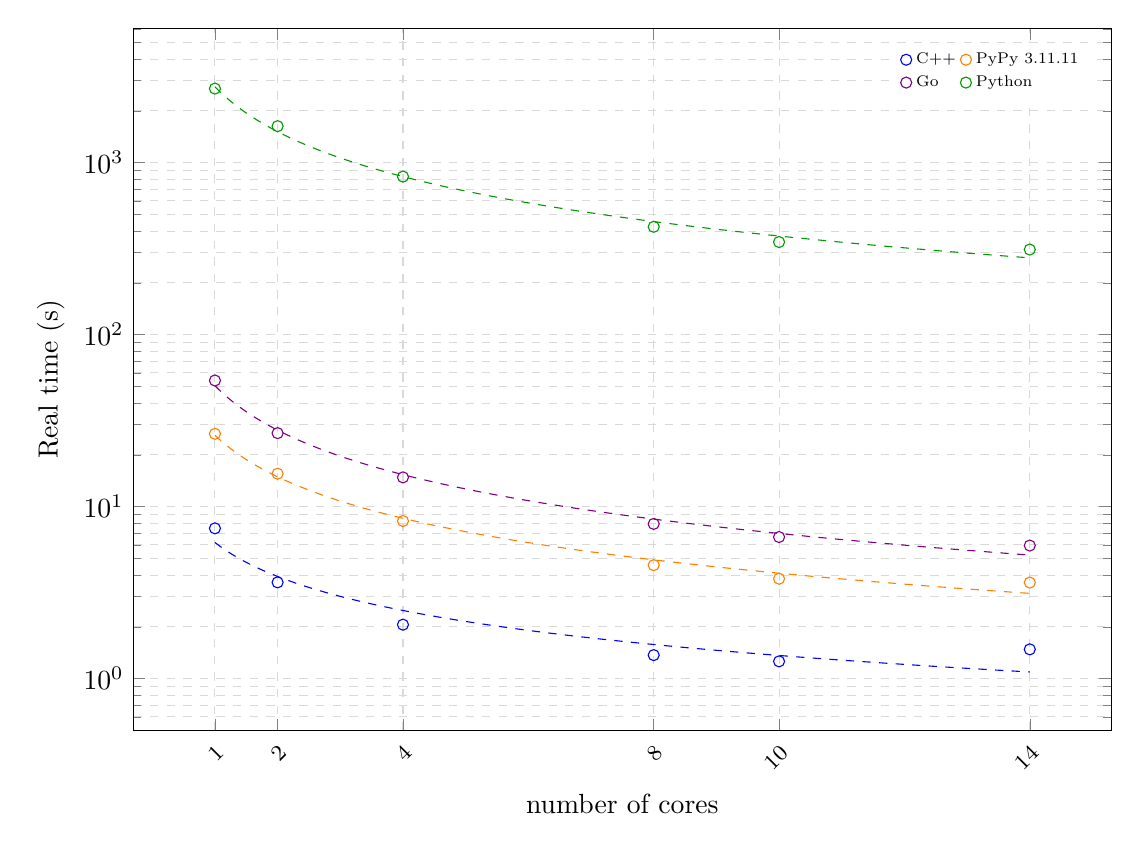
\begin{tikzpicture}
  \begin{semilogyaxis}[
      width=14cm,
      height=10.5cm,
      xlabel={number of cores},
      ylabel={Real time (s)},
      ymode=log,
      xmode=linear,
      grid=both,
      minor tick num=1,
      grid style={gray!30,dashed},
      xtick={1,2,4,8,10,14},
      x tick label style={
        font=\footnotesize,
        rotate=45,
        anchor=north east
      },
      legend style={
        at={(0.98,0.98)},
        anchor=north east,
        font=\scriptsize,
        nodes={scale=0.8,transform shape},
        draw=none
      },
      legend columns=2,
      transpose legend,
      legend cell align=left,
    ]
    %% C++ %%
    \addplot[
      blue,
      only marks,
      mark=o,
      mark options={draw=blue,fill=white}
    ]
    table[row sep=\\] {
      x   y     \\
      1   7.48  \\
      2   3.63  \\
      4   2.06  \\
      8   1.37  \\
      10  1.26  \\
      14  1.48  \\
    };
    \addlegendentry{C++}
    % power‐law fit: y = 6.19 * x^(–0.657)
    \addplot[
      blue,
      dashed,
      forget plot,
      domain=1:14,
      samples=200
    ] {6.19 * x^(-0.657)};

    %% Go %%
    \addplot[
      violet,
      only marks,
      mark=o,
      mark options={draw=violet,fill=white}
    ]
    table[row sep=\\] {
      x   y      \\
      1   54.16  \\
      2   26.76  \\
      4   14.80  \\
      8   7.94   \\
      10  6.66   \\
      14  5.94   \\
    };
    \addlegendentry{Go}
    % power‐law fit: y = 50.5 * x^(–0.859)
    \addplot[
      violet,
      dashed,
      forget plot,
      domain=1:14,
      samples=200
    ] {50.5 * x^(-0.859)};

    %% PyPy 3.11.11 %%
    \addplot[
      orange,
      only marks,
      mark=o,
      mark options={draw=orange,fill=white}
    ]
    table[row sep=\\] {
      x   y      \\
      1   26.52  \\
      2   15.55  \\
      4   8.25   \\
      8   4.57   \\
      10  3.81   \\
      14  3.62   \\
    };
    \addlegendentry{PyPy 3.11.11}
    % power‐law fit: y = 26.0 * x^(–0.802)
    \addplot[
      orange,
      dashed,
      forget plot,
      domain=1:14,
      samples=200
    ] {26.0 * x^(-0.802)};

    %% Python %%
    \addplot[
      green!60!black,
      only marks,
      mark=o,
      mark options={draw=green!60!black,fill=white}
    ]
    table[row sep=\\] {
      x    y       \\
      1    2697.08 \\
      2    1631.14 \\
      4    830.61  \\
      8    423.92  \\
      10   345.83  \\
      14   312.64  \\
    };
    \addlegendentry{Python}
    % power‐law fit: y = 2765 * x^(–0.868)
    \addplot[
      green!60!black,
      dashed,
      forget plot,
      domain=1:14,
      samples=200
    ] {2765 * x^(-0.868)};

  \end{semilogyaxis}
\end{tikzpicture}

    \caption{Execution time of the MPB example in different programming languages.}
    \label{fig:mpb-execution-time}
\end{figure}

\begin{table}
    \centering
    \begin{tabular}{lrrrr}
        \hline
        Cores & C++  & Go    & PyPy 3.11.11 & Python    \\
        \hline
        1     & 7.48  & 54.16  & 26.52        & 2,697.08  \\
        2     & 3.63  & 26.76  & 15.55        & 1,631.14  \\
        4     & 2.06  & 14.80  & 8.25         & 830.61    \\
        8     & 1.37  & 7.94   & 4.57         & 423.92    \\
        10    & 1.26  & 6.66   & 3.81         & 345.83    \\
        14    & 1.48  & 5.94   & 3.62         & 312.64    \\
        \hline
    \end{tabular}
    \caption{Real execution time by implementation and core count}
    \label{tab:real-execution}
\end{table}

\subsection{Raspberry Pi 5}
\subsubsection{Evaluated parameters}
\subsubsection{Results}


\section{Comment on paralellizing different languages}

In this section, I would like to make some comment on the paralelization on different languages, and why some might experience a different behaviour. 

\subsection{Go}
When choosing how many "cores" the tests are using, for the Go implementation, I used the size of the \texttt{waitChan} channel. This number can be changed to be more than the total number of threads in the system, which sometimes increases the performance.

\begin{table}
  \centering
  \begin{tabular}{lccc}
    \toprule
    Cores & Goroutines & Energy consumed (pkg) & Execution time \\
    \midrule
    1             & 1          &  28,522.69     &   172.95  \\ 
    1             & 2          &  28,919.31     &   175.38  \\ 
    2             & 2          &  18,231.97     &   89.319  \\
    2             & 4          &  18,224.50     &   89.275  \\
    4             & 4          &  10,304.27     &   45.508  \\
    4             & 8          &  10,299.06     &   45.482  \\
    8             & 8          &  5,617.27      &   23.781  \\
    8             & 16         &  5,580.52      &   23.594  \\
    14            & 14         &  3,155.30      &   14.034  \\
    14            & 28         &  3,151.93      &   14.001  \\
    16            & 16         &  2,904.52      &   12.456  \\
    16            & 32         &  3,018.54      &   12.435  \\
    28            & 28         &  2,306.35      &   8.9061  \\
    28 Same CPU   & 28         &  2,271.71      &   7.6137  \\
    28            & 56         &  2,314.29      &   7.7914  \\
    28 Same CPU   & 56         &  2,290.85      &   8.8153  \\
    32            & 32         &  2,151.74      &   8.1632  \\
    32 Same CPU   & 32         &  2,109.37      &   6.8224  \\
    32            & 64         &  2,121.88      &   8.1017  \\
    32 Same CPU   & 64         &  2,142.21      &   6.8960  \\
    48            & 48         &  1,856.93      &   5.7187  \\
    48            & 96         &  1,848.47      &   5.6737  \\
    60            & 60         &  1,744.76      &   5.3571  \\
    60            & 120        &  1,737.80      &   5.3208  \\
    60            & 200        &  1,724.73      &   5.2556  \\
    60            & 250        &  1,719.49      &   5.2182  \\
    \bottomrule
  \end{tabular}
  \caption{Go goroutines and threads used in the tests}
  \label{tab:go-routines-cores}
\end{table}

As it can be seen from \autoref{tab:go-routines-cores}, the Go implementation is able to use more than the total number of threads in the system, and it is able to use them efficiently, as the Go runtime is able to schedule the goroutines efficiently.

\subsection{Python}
When iterating though every pixel in Python, as the environment has to be copied for every single pixel, the cores are not being used at 100\% of their capacity, specifically, while testing I saw that the cores were being used at around 5\% of their capacity. Meaning the creation of too many threads is not beneficial, as the overhead of creating the threads is larger than the actual work being done by each thread. 
Another factor that Python, each time a task is submitted to a process, Python needs to serialize (pickle) the entire world object and other parameters, then deserialize them in the worker process, which means that, if this has to happen for every pixel, the serializing and deselializing tasks run for much longer than the actual pixel processing.

\section{Most efficient language optimizations}
As we can see from these results, the most efficient language in terms of energy consumption and execution time is C\++. 

But, out of the box, does C++ always provide the best performance? The answer is no, as the compiler plays an extremely important role in the performance of the code, and the compiler optimizations can make a huge difference in the performance of the code.
For these tests, I many optimization flags, such as \texttt{-O3} and \texttt{-march=native}, which allows the compiler to optimize the code for the specific architecture of the machine it is being compiled on. But what would happen if we used different compiler flags, would the results change? Would another language be more efficient?

As to not leave the reader with the intreague of what would happen if we used different compiler flags, I have compiled and tested all the programs with the following flags:
\begin{itemize}
    \item \texttt{-O0}: No optimizations, the compiler will not optimize the code at all.
    \item \textbf{-O1}: Basic optimizations; the compiler will optimize the code. It performs a basic cleanup, removing dead code and some simple inlining.
    \item \textbf{-O2}: More optimizations; this is the recommended optimization level for most use cases.
    \item \textbf{-O3}: Maximum optimizations, very aggressive optimizations:
    \begin{itemize}
        \item Loop transformations: Unrolling loops even more than \texttt{-O2}, changing the distribution of loops and interchanging them.
        \item Speculative optimizations
        \item Vectorization: \gls{SIMD} instructions (AVX, SSE, etc.)
        \item Predictive commoning (reuses computations from previous loop iterations)
    \end{itemize}
    \item \textbf{-O3 with --fast-math}: Maximum optimizations; the compiler will optimize the code as much as possible, but operations will not be as precise.
\end{itemize}

As \autocite{llvm-fast-math} explains, the \texttt{--fast-math} flag allows the compiler to perform optimizations that may not be mathematically correct, but will result in faster code. 


\begin{table}
  \centering
  \begin{tabular}{lrrrrr}
    \toprule
    \textbf{Metric / Flags} & \textbf{-O0} & \textbf{-O1} & \textbf{-O2} & \textbf{-O3} & \textbf{-O3 (fast-math)} \\
    \midrule
    \multicolumn{6}{c}{\textbf{1 core}} \\
    power/energy-pkg (J) & 52,957.47 & 5,185.28 & 4,388.12 &  4,031.83   & \textbf{4,005.70} \\
    power/energy-ram (J) & 2,208.08  & 210.28   & 183.21   &    180.00   & \textbf{168.52}  \\
    time (s)             & 270.06    & 27.453   & 24.02    &     23.5993 & \textbf{22.054}  \\
    \midrule
    \multicolumn{6}{c}{\textbf{4 cores}} \\
    power/energy-pkg (J) & 13,379.59 & 1,564.51 & 1,417.01 & \textbf{1,386.60} & 1,414.08       \\
    power/energy-ram (J) & 508.40    & 56.72    & 50.96    &     50.37         & \textbf{49.56}  \\
    time (s)             & 66.066    & 7.4351   & 6.67     &    6.5605         & \textbf{6.478}  \\
    \midrule
    \multicolumn{6}{c}{\textbf{14 cores}} \\
    power/energy-pkg (J) & 5,056.15  & 658.46   & 606.58   & \textbf{595.29}  & 639.00         \\
    power/energy-ram (J) & 153.03    & 20.79    & 18.53    & \textbf{18.24}  & 20.10          \\
    time (s)             & 19.9344   & 2.7184   & 2.42     & \textbf{2.3807} & 2.62           \\
    \midrule
    \multicolumn{6}{c}{\textbf{28 cores}} \\
    power/energy-pkg (J) & 3,650.43  & 627.89   & 565.83   &    561.59   & \textbf{547.56} \\
    power/energy-ram (J) & 120.49    & 20.00    & 18.00    &     17.93   & \textbf{17.47}  \\
    time (s)             & 15.729    & 2.6043   & 2.36     &     2.3382  & \textbf{2.2701} \\
    \midrule
    \multicolumn{6}{c}{\textbf{32 cores}} \\
    power/energy-pkg (J) & 3,353.53  & 606.52   & 552.98   &     548.83  & \textbf{535.22} \\
    power/energy-ram (J) & 110.47    & 19.54    & 17.76    &     17.58   & \textbf{17.27}  \\
    time (s)             & 14.4472   & 2.5369   & 2.33     &     2.3015  & \textbf{2.2368} \\
    \midrule
    \multicolumn{6}{c}{\textbf{60 cores}} \\
    power/energy-pkg (J) & 2,794.03  & 698.96   & 661.76   & \textbf{659.31} & 671.51         \\
    power/energy-ram (J) & 86.80     & 25.37    & 24.11    & \textbf{24.10}  & 24.76          \\
    time (s)             & 7.5463    & 1.89955  & 1.80     &     1.79288     & \textbf{1.79288}\\
    \bottomrule
  \end{tabular}
  \label{tab:compiler-optimizations}
    \caption{Power/Energy and execution time for various core counts and compiler optimization flags. Boldface indicates the minimum value in each row.}
\end{table}

From the \autoref{tab:compiler-optimizations}, we can see that -O3 can be upto $13.13x$ mroe efficient and $11.44x$ faster than \texttt{-O0}, and \texttt{-O3} and $13.22x$ more efficient and $12.25x$ faster if we add the \texttt{--fast-math} flag on a single core task. But when we change and add more cores, the improvement decreases up to $4.24x$ faster more energy efficient and $4.16x$ faster with \texttt{-O3} and consume $4.22x$ less energy and take $4.11x$ less time with \texttt{-O3 --fast-math}.

Thus, we can see that the compiler optimizations play a very important role in the performance of the code, and that C\++ is not always the most efficient language, as it depends on the compiler optimizations used. In conclusions, for optimization flags, eventhough \texttt{-O3 with --fast-math} is the most efficient, I would recommend using \texttt{-O3} for high-performance computing, as it provides a good balance between performance and accuracy. If the program is just a regular program, I would recommend using \texttt{-O2}, as it provides a good balance between performance and code size as well as compilation time, which we have not taken into account as the program is just compiled once and may be executed thousands of times.